\documentclass[../Report.tex]{subfiles}
\graphicspath{ {../../Images/} }
\begin{document}
    \chapter{Ricerca Etnografica}
    \section{Segmentazione}
    Una piattaforma di gioco come gioco.it non riguarda le esigenze primarie di un bambino, potremmo comunque identificarlo nel penultimo livello della piramide di Maslow: Stima del gruppo e auto-attualizazzione.
    Lo possiamo considerare come un momento di divertimento e di sfida in modo che possa permettere all’utente di qualunque etá di giocare alla piattaforma in modo sicuro, indipendentemente dall’eta, specifiche del computer ecc.
    Il sito puó essere anche usato per allenare le proprie capacitá di problem solving, creativitá e apprendimento.

    \subsection{Segmentazione Demografica}
    
    Non esiste una specifica distinzione a priori tra soggetti per un gruppo demografico maschile o femminile poiché il sito si rivolge ad entrambi cerchiamo tuttavia però di distinguere gli utilizzatori attraverso l’eta:
    \begin{itemize}
        \item Bambini (6-14): primi approcci ad un computer, potrebbero essere interessati anche a giochi di tipo educativo
        \item Adolescenti (14-22):il sito è di facile accesso tramite qualsiasi browser [per ammazzare la noia]
        \item Adulti ($\>$22): Durante un’attesa persone abituate ai videogiochi potrebbero essere utenti target per questa piattaforma
    \end{itemize}

    Illustriamo attraverso il seguente grafico alcune considerazioni intuitive tra il rapporto di età di un utente,il tempo libero che un individuo possiede e il tempo di utilizzo del nostro servizio. 
    È una stima indicativa per evidenziare il target di utenti piu adatto su cui focalizzarci.
    Assumiamo che la fascia 5-10/10-18 sia quella con maggior tempo libero a disposizione e con predisposizione tale da utilizzare il nostro servizio, la fascia di mezzo (30-60) è quella con minor tempo libero, di conseguenza, con il minor tempo di utilizzo ed infine la fascia $\>$65 il tempo libero aumenta però l’utilizzo di una piattaforma di giochi online è veramente ridotto. 

    \begin{figure}{H}
        \centering
        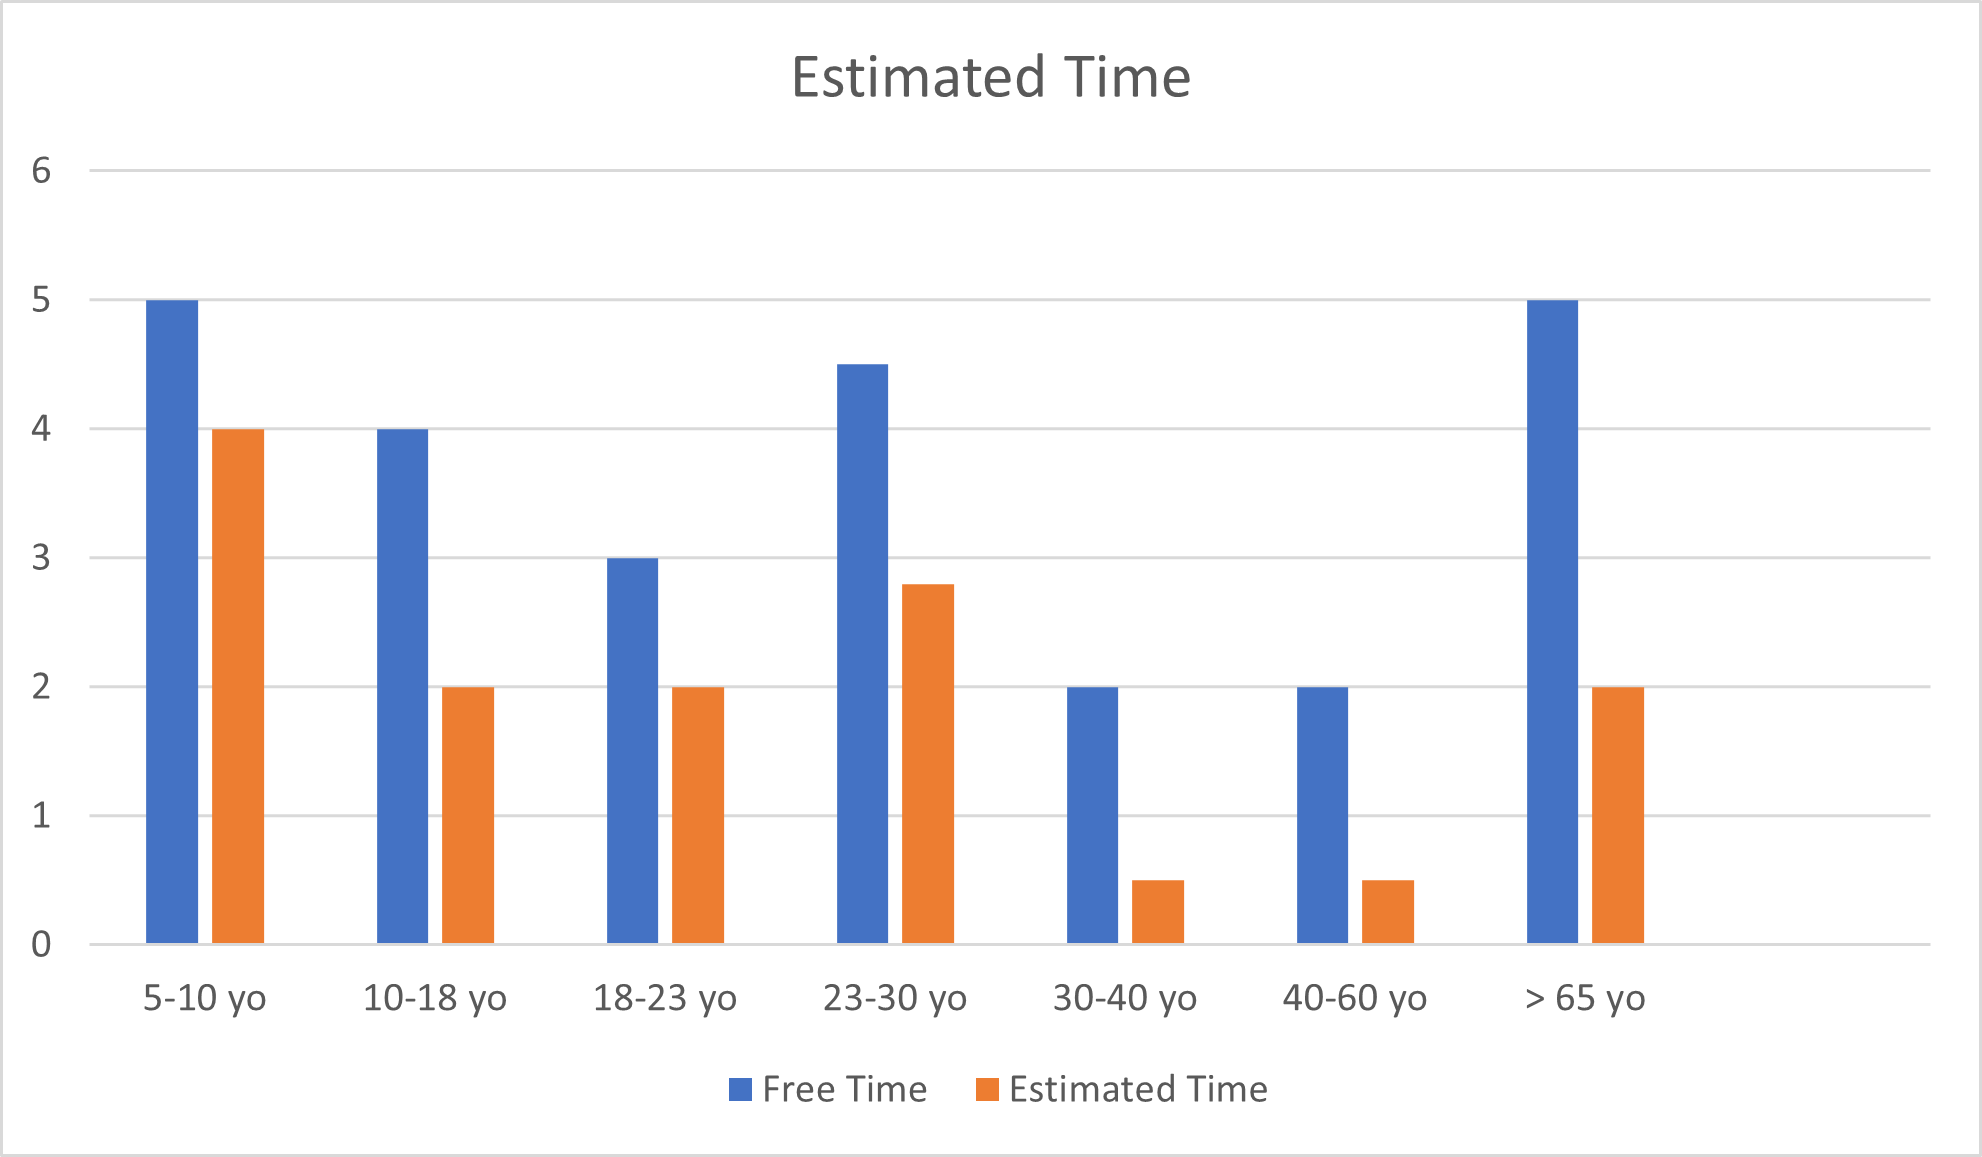
\includegraphics{EstimatedTime.png}
    \end{figure}

    Nel prossimo grafico invece mostreremo una stima delle competenze in ambito informatico in base alle differenti fasce d’eta, distinguendo le ‘Competenze’ tra basse (accendere/spegnere un computer, navigare nel dekstop, controllare la mail), medie(scaricare applicazioni, utilizzare un word processor e fogli di calcolo),alte(ottima familiaritá con l’utilizzo dei computer).

    \begin{figure}[H]
        \centering
        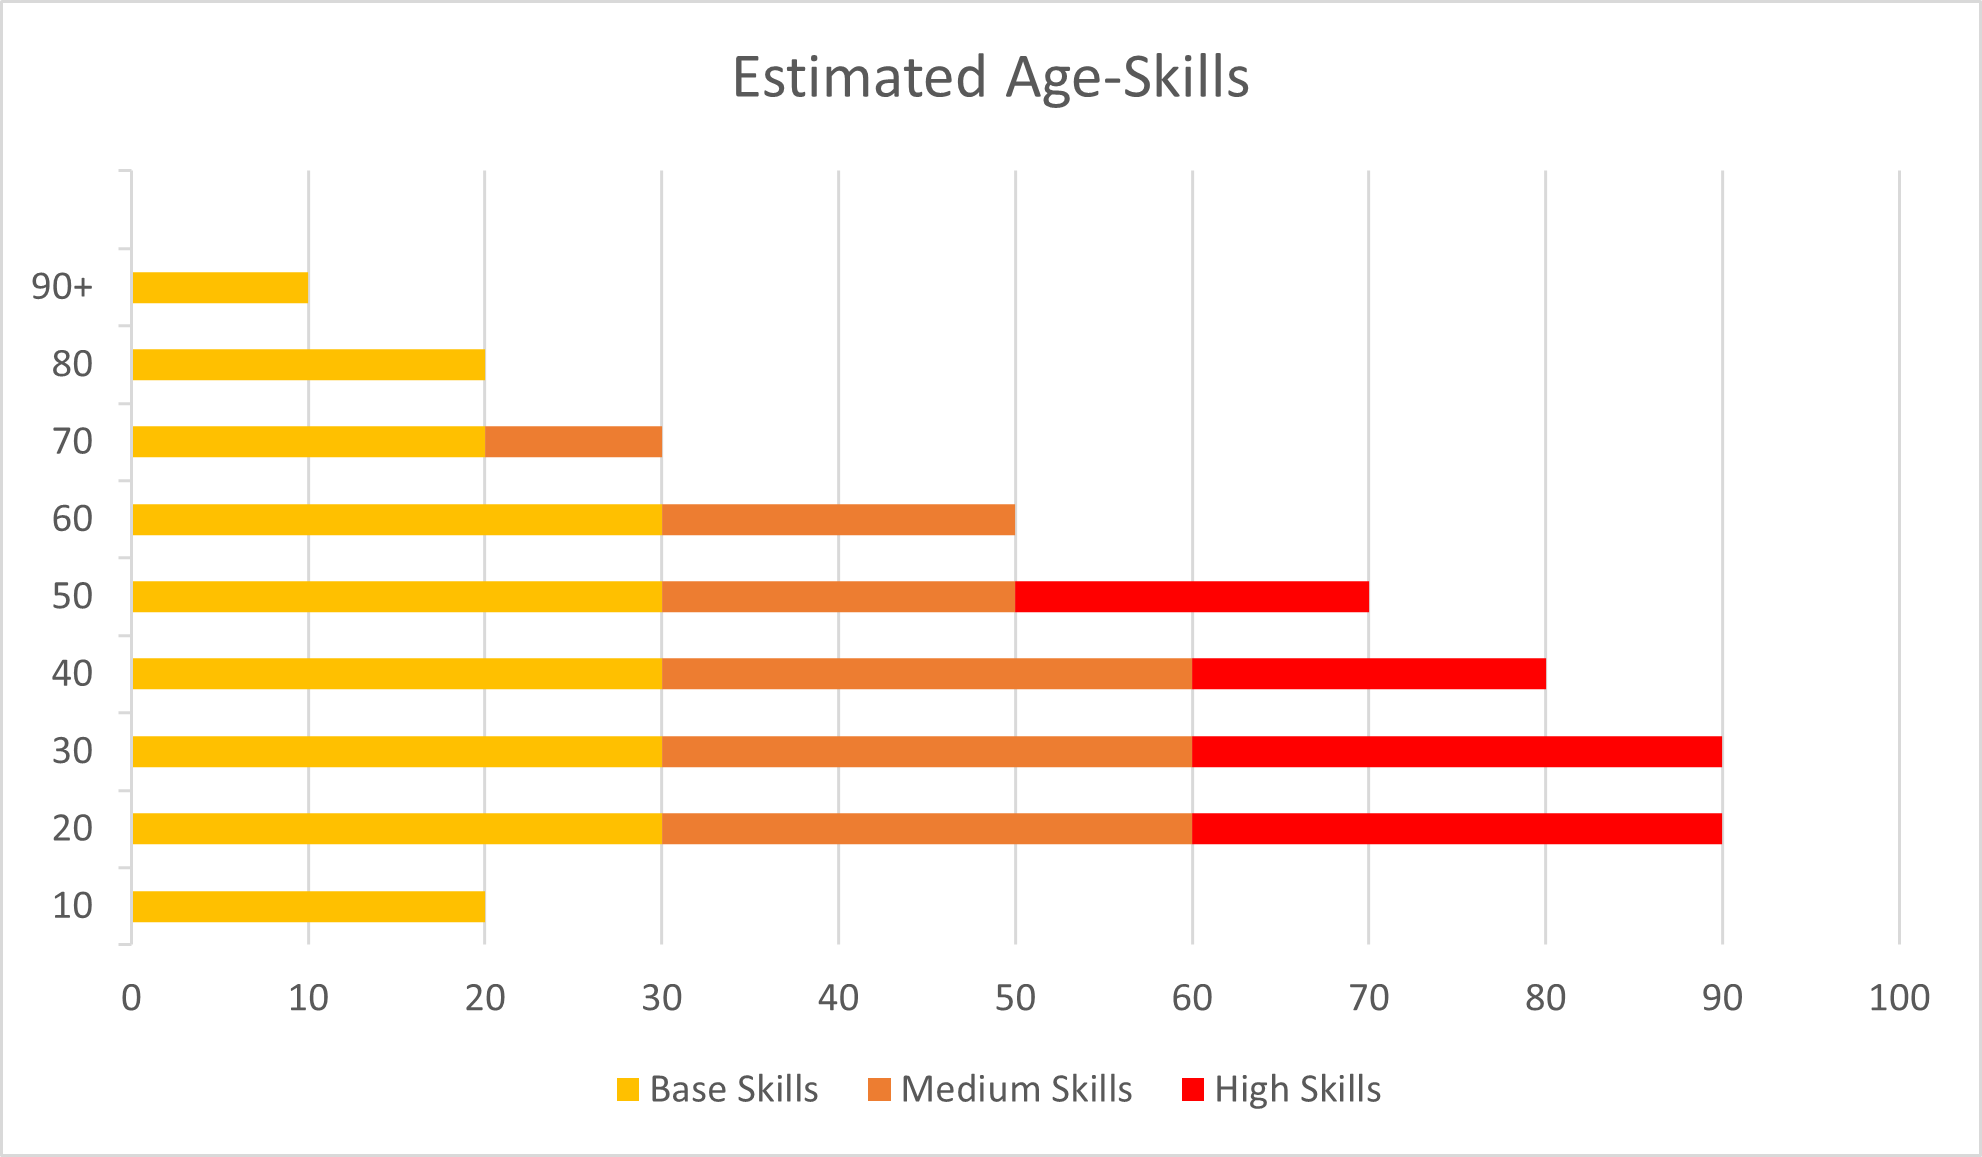
\includegraphics{EstimatedAgeSkills.png}
    \end{figure}

    Intuitivamente possiamo capire che le persone tra 20-40 anni possiedono in media piú competenze e abilitá nell’utilizzo dei computer mentre troviamo piú difficolta nella fascia attorno ai 10 anni e \>80.
    \subsection{Segmentazione Psicografica}

    Non ci sono tratti psicologici distintivi, ma magari un breve periodo monotono e tedioso può incontrare nel sito un ottimo spunto di favore.
    Non avendo una segmentazione demografica netta l’interfaccia dovrà conciliare i gruppi di età degli utenti proponendo descrizioni, giudizi di altri utenti in modo da rendere il gruppo di utenti sempre più ampio (fattore molto utile per quanto riguarda la possibilità del multiplayer).

    \subsection{Segmenti Target}
    Identifichiamo così possibili segmenti target:
    \begin{itemize}
        \item Genitori o parenti di un utente bambino (3-18 anni) i quali apro il browser e si collegano al sito, gli verrà illustrato come funziona il gioco e il bambino imparerà a giocarci. Il bambino in questo caso non ha competenze informatiche, è tra i primi momenti in cui approccia ad un computer non è in grado di raggiungere il sito e muoversi all’interno di esso.
        \item Adulti (30-50 anni) Utenti maggiorenni, con competenze informatiche di ogni genere, l’abilità dell’interfaccia sará anche quella di fornire un’interfaccia efficiente sia per persone anziane poco esperte all’utilizzo di computer e utenti più giovani in grado di usarlo molto bene.      
    \end{itemize}

    \section{Ricerca Utenti}
    
    La nostra ricerca sugli utenti consiste in interviste con campioni di utenti scelti dai nostri dati demografici.\\
    In questa sezione il nostro obiettivo è determinare:
    \begin{itemize}
        \item Se i segmenti provvisori della sezione precedente rispondono bene all’idea alla base del nostro e costituiscono un buon pubblico di destinazione
        \item Evidenziare le principali aspettative degli utenti target per quanto riguarda l’utilizzo della piattaforma
    \end{itemize}

    
    \subsection{interviste}
    Descriviamo la nostra ipotetica piattaforma ai nostri intervistati e poniamo loro una serie di domande riguardanti l’argomento:
   
    \begin{enumerate}
    \item Hai buona familiarità con l’utilizzo dei computer e dei sistemi informatici?
    \item Hai mai giocato su internet in una piattaforma di giochi online?
    \item Pensi che vorrai utilizzare il servizio?\\
        \hrule In caso affermativo\\
        \begin{enumerate}
            \item Quando pensi che potresti utilizzare il servizio?\\ \hrule In caso negativo: 
            \item Come mai?
            \item Chi pensi possa essere più adeguato ad utilizzare questo servizio?
        \end{enumerate}
    \item	Quali pensi possano essere i vantaggi pi significativi di questo servizio?
    \item	Quali pensi possano essere i vantaggi meno significativi di questo servizio?
    \item	Pensi che ci possa essere qualche preoccupazione nell’utilizzo della piattaforma da utenti minorenni?
    \end{enumerate}

    \subsubsection{Risultati:}
    
    \textbf{Intervistato A}

    \textbf{Nome}:Sofia\\
    \textbf{Eta'}:36\\
    \textbf{Professione}:Impiegata\\
    
    \begin{enumerate}
        \item Buona familiarità con l’utilizzo degli strumenti informatici dovuto ad un forte utilizzo in ambito lavorativo e personale
        \item Si, ha giocato in momenti morti e vede spesso i suoi figli (6 e 12 anni) giocarci 
        \item Probabilmente si, per riempire momenti morti oppure farli giocare ai figli per scopi educativi.
        \item La presenza di un filtro che permette ai bambini di giocare solo ai giochi adeguati alla sua età la fa farebbe stare tranquilla come mamma.
        \item Nessuna risposta
        \item No, però serve un’attenzione da parte dei genitori per fare in modo che i filtri non vengano ignorati dai bambini
    \end{enumerate}

    Note: Di solito per cercare questo tipo di giochi guarda i primi risultati delle ricerche su Google\\

    \hrule
    \textbf{Intervistato B}

    \textbf{Nome}:Gianni\\
    \textbf{Eta'}:63\\
    \textbf{Professione}:Libero Professionista\\
    
    \begin{enumerate}
        \item Scarsa conoscenza dei sistemi informatici, usa il telefono per rispondere a chiamate di lavoro
        \item Non ha mai giocato sui giochi di piattaforma online però ha visto i suoi figli (15 e 23 anni) giocarci
        \item Non crede ci giocherebbe date le competenze informatiche limitate, ha un computer a casa che lo usano principalmente la moglie e i figli. \\Pensa che sarebbe piú adeguato un pubblico piú giovane che abbia maggior conoscenza dei sistemi informatici
        \item Il fatto che i giochi siano liberamente accessibili potrebbero essere un vantaggio
        \item Il piú grande svantaggio potrebbe essere che molte recensioni possano essere false per aumentare la visibilitá di un determinato gioco
        \item Secondo lui si perche i bambini in casi come questo giocherebbero troppo e sarebbero troppo esposti all'utilizzo del computer
        
    \end{enumerate}
    \hrule
    \textbf{Intervistato C}\\
    
    \textbf{Nome}:Fabrizio\\
    \textbf{Eta'}:38\\
    \textbf{Professione}:Operaio\\

    \begin{enumerate}
        \item Limitata conoscenza de computer, utilizza solo lo smartphone per chiamare, mandare messaggi e navigare sui social network
        \item Si, sui giochi online dei social network quale facebook, con le sfide con gli amici
        \item Gli piacerebbe prendere dimestichezza con i computer, in caso contrario potrebbe provare a far giocare il figlio (8 anni) se avesse la sicurezza di giocare in un ambiente ‘sicuro’
        \item Avere per ogni gioco una descrizione e una valutazione fornita da altri utenti 
        \item Non ha molta fiducia nel filtro per minori
        \item Non crede, per il fatto delle recensioni da altri utenti possano difficilmente essere surreali
    \end{enumerate}

    \hrule
    \textbf{Intervistato D}\\

    \textbf{Nome}:Sara\\
    \textbf{Eta'}:23\\
    \textbf{Professione}:Studentessa universitaria\\

    \begin{enumerate}
        \item Buone competenze digitali dovuto ad un assidio utilizzo in universita e a casa
        \item Si, diverse volte soprattutto nelle lezioni in laboratorio o comunque quando deve prendersi una pausa dallo studio
        \item Sì, però solo nei momenti morti (pausa studio o noia), non accenderebbe mai il computer per utilizzare la piattaforma
        \item Il fatto che sia accessibile da piu dispositivi e non servono requisiti e competenze avanzate puo essere un punto favorevole
        \item Le descrizioni e l’immagine che descrivono i giochi nella pagina principale devono essere chiare per non far perdere tempo a provare giochi poco interessanti
        \item Si, poiché tanto i divieti vengono ignorati quindi se un bambino vuole ignorare il filtro riuscirá benissimo a farlo senza problemi
        
    \end{enumerate}

    \hrule
    \textbf{Intervistato E}\\

    \textbf{Nome}:Lucia\\
    \textbf{Eta'}:44\\
    \textbf{Professione}:Insegnante delle elementari\\

    \begin{enumerate}
        \item Buona familiaritá con l’uso dei computer dovuto ad un uso quotidiano durante l’orario scolastico e al di fuori di esso per uso personale
        \item Non ha mai giocato su questo tipo di piattaforme ma potrebbe essere utile da far giocare agli studenti magari per giochi a scopo educativo e durante l’ora di laboratorio di informazione
        \item Userebbe il servizio nel suo tempo libero per vedere come mostrarlo ai bambini poi in caso di riscontro positivo, farebbe giocare i bambini durante l’orario di laboratorio
        \item Dal suo punto di vista i filtri per l’eta e le categorie di giochi sono i vantaggi piu importanti e in caso lo strumento di cui fará maggior affidamento durante la valutazione del servizio e dei giochi stessi
        \item Il fatto che non si possa stilare un ranking tra un determinato gruppo di utenti
        \item Non crede che l’utilizzo di questo servizio da parte di studenti minorenni controllati da un adulto possano destare preoccupazioni
    \end{enumerate}
    \hrule
    \textbf{Intervistato F}\\
    
    \textbf{Nome}:Luca\\
    \textbf{Eta'}:21\\
    \textbf{Professione}:Studente Universitario\\

    \begin{enumerate}
        \item Ottima conoscenza dei sistemi informatici, utilizzo dei social network e fa spesso ricerche in ambito accademico
        \item Si, spesso per prendere una pausa dallo studio cerca dei siti dove si puo giocare online non sforzando troppo la testa
        \item Si, potrebbe fare al caso suo; soprattutto quando dovrebbe staccare la testa dallo studio
        \item Che sia facilmente accessibile da un browser, non richieda plug in particolari o accessori sofisticati
        \item Spesso i giochi possono essere noiosi, serve che le recensioni e le descrizioni siano ben visibile e soprattutto veritiere
        \item Beh, sicuramente deve esistere un filtro perché anche in giochi ‘semplici’ possono esserci contenuti non adeguati ad un pubblico minorenne
    \end{enumerate}
    
    \textbf{Intervistato G}\\
    \hrule
    \textbf{Nome}:Andrea\\
    \textbf{Eta'}:32\\
    \textbf{Professione}:Impiegato\\

    \begin{enumerate}
        \item Buona conoscenza dei sistemi informatici, utilizza il computer per scopi lavorativi
        \item No, dato che non ha un computer a casa e l’unico strumento sarebbe dal computer del lavoro in cui non è possibile per le policy aziendali 
        \item Risulta decisamente complicato per la mancanza di dispositivi, magari se fosse presente una versione mobile potrebbe provarla ma è consapevole che l’usabilitá a giocare da browser su un dispositivo mobile sarebbe totalmente diversa rispetto a scaricare un’applicazione ad-hoc
        \item Non sa rispondere
        \item L’usabilita di giocare tramite un browser è diversa da giocare in locale, potrebbe essere un punto a sfavore
        \item \textit{Non sa rispondere}    
    \end{enumerate}

    \newpage
    \subsection{Conclusioni}

    Notiamo che le interviste hanno confermato la validitá dei nostri dati demografici e psicografici, poiché tutti gli intervistati hanno espresso interesse nell’uso del servizio o un interessamento allo stesso.
    Inoltre, da queste interviste possiamo risaltare una lista di casi d’uso provvisori che ci mettono in evidenzia il ‘perché’ debba utilizzare il nostro servizio, e troviamo:
    \begin{itemize}
        \item Motivi di svago e distrazione
        \item Motivi Educativi
    \end{itemize}
    Abbiamo inoltre focalizzato l’attenzione sugli utenti target che ci sembrano tutt’ora una cerchia che rispettano pienamente la clientela del sito.\\
    Da un’osservazione delle interazioni degli utenti abbiamo notato inoltre che:
    \begin{itemize}
        \item Un gioco deve essere ben descritto, avere delle chiare immagini esemplificative e avere delle recensioni veritiere
        \item La schermata deve essere intuitiva, l’utente usa il servizio e gioca per un periodo limitato di tempo; deve essere invogliato a scegliere il miglior gioco nel minor tempo possibile
        \item Di solito i genitori che accompagnano i figli nel gioco non sono abili nell’uso dei computer, bisogna dare la possibilitá anche a loro di usare il sito
    \end{itemize}
    L’utilizzo del servizio da parte di utenti minorenni non sembra destare molta preoccupazione, nonostante si è consapevoli che il filtro potrebbe essere bypassato come servizio bisognerebbe cercare di ottimizzarla al meglio, ma il controllo da parte dei genitori sembra comunque essenziale.

    \subsubsection*{Altre Idee}
    Dalle interviste, tuttavia, sono venute fuori particolari funzionalitá che potrebbero essere aggiunte in futuro:
    \begin{itemize}
        \item Avere una sezione contenenti le classifiche dei giochi piu utilizzati e in base alla valutazione degli utenti
        \item Possibilitá di connettere un gruppo di amici, ed eventualmente stilare le varie classifiche
        \item Limitare il tempo di gioco di un utente minorenne sotto la supervisione di un genitore
        
    \end{itemize}



\end{document}